% !TeX spellcheck = en_US


\chapter{Relevant Works}

\section{Passive Whisker Sensors}

\section{Active Tactile Exploration}

\subsection{3D Mapping of Underground Mining Environments}
\begin{columns}[T,onlytextwidth]
    \begin{column}[T]{0.48\textwidth}
        \begin{figure}[H]
            \centering
            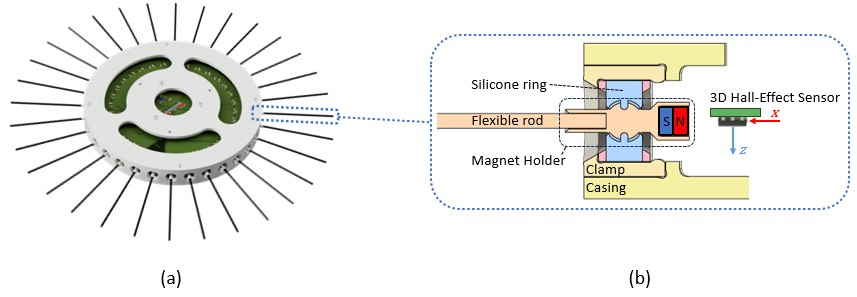
\includegraphics[width=\textwidth]{figures/related-works-1-prototype}
            \caption{Whisker disk prototype. (a) The sensor comprises a circular array of 32 whiskers. (b) Detailed section view of a single whisker sensor, from~\cite{biomimetics9020083}}
        \end{figure}
    \end{column}
    \begin{column}[T]{0.48\textwidth}
        \begin{figure}[H]
            \centering
            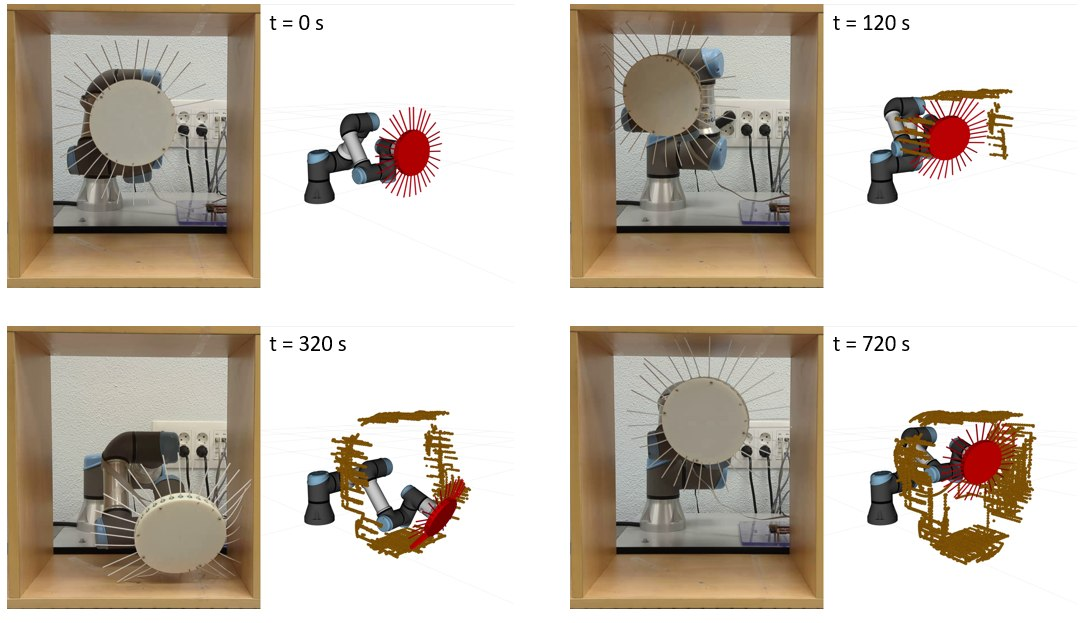
\includegraphics[width=\textwidth]{figures/related-works-1-results}
            \caption{Environment reconstruction from the 3D-mapping experiment, from ~\cite{biomimetics9020083}}
        \end{figure}
    \end{column}
\end{columns}

\subsection{Active Tactile Exploration}
\textbf{Whisker sensors per se are passive sensors. \to Active control is required.}\\
\begin{columns}[T,onlytextwidth]
    \begin{column}[T]{0.48\textwidth}
        \begin{figure}[H]
            \centering
            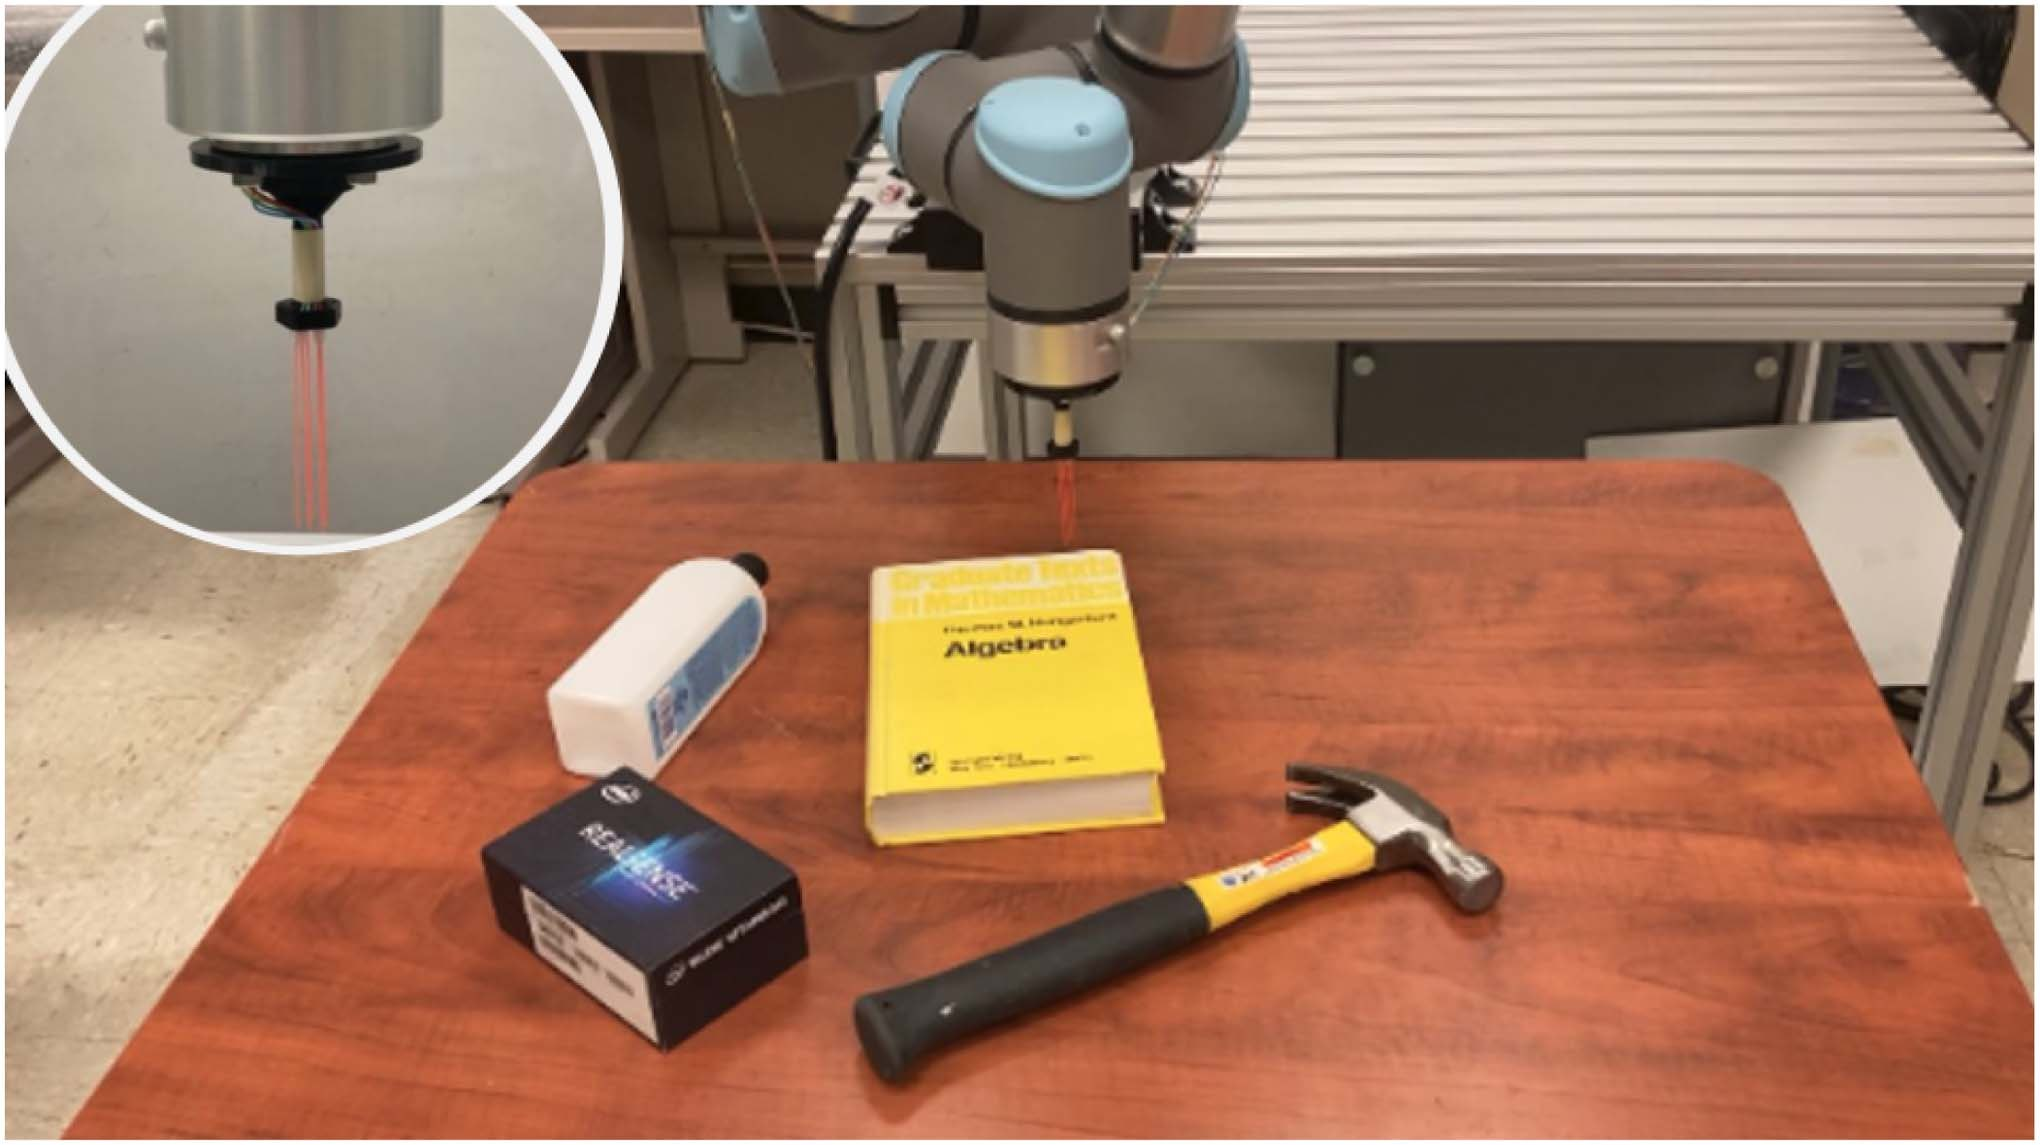
\includegraphics[width=\textwidth]{figures/related-works-2-prototype}
            \caption{Robot is using the tactile feedback from our developed whisker sensor to localize, and recognize the objects found during exploration, from~\cite{Xiao_2022}}
        \end{figure}
    \end{column}
    \begin{column}[T]{0.48\textwidth}
        \begin{figure}[H]
            \centering
            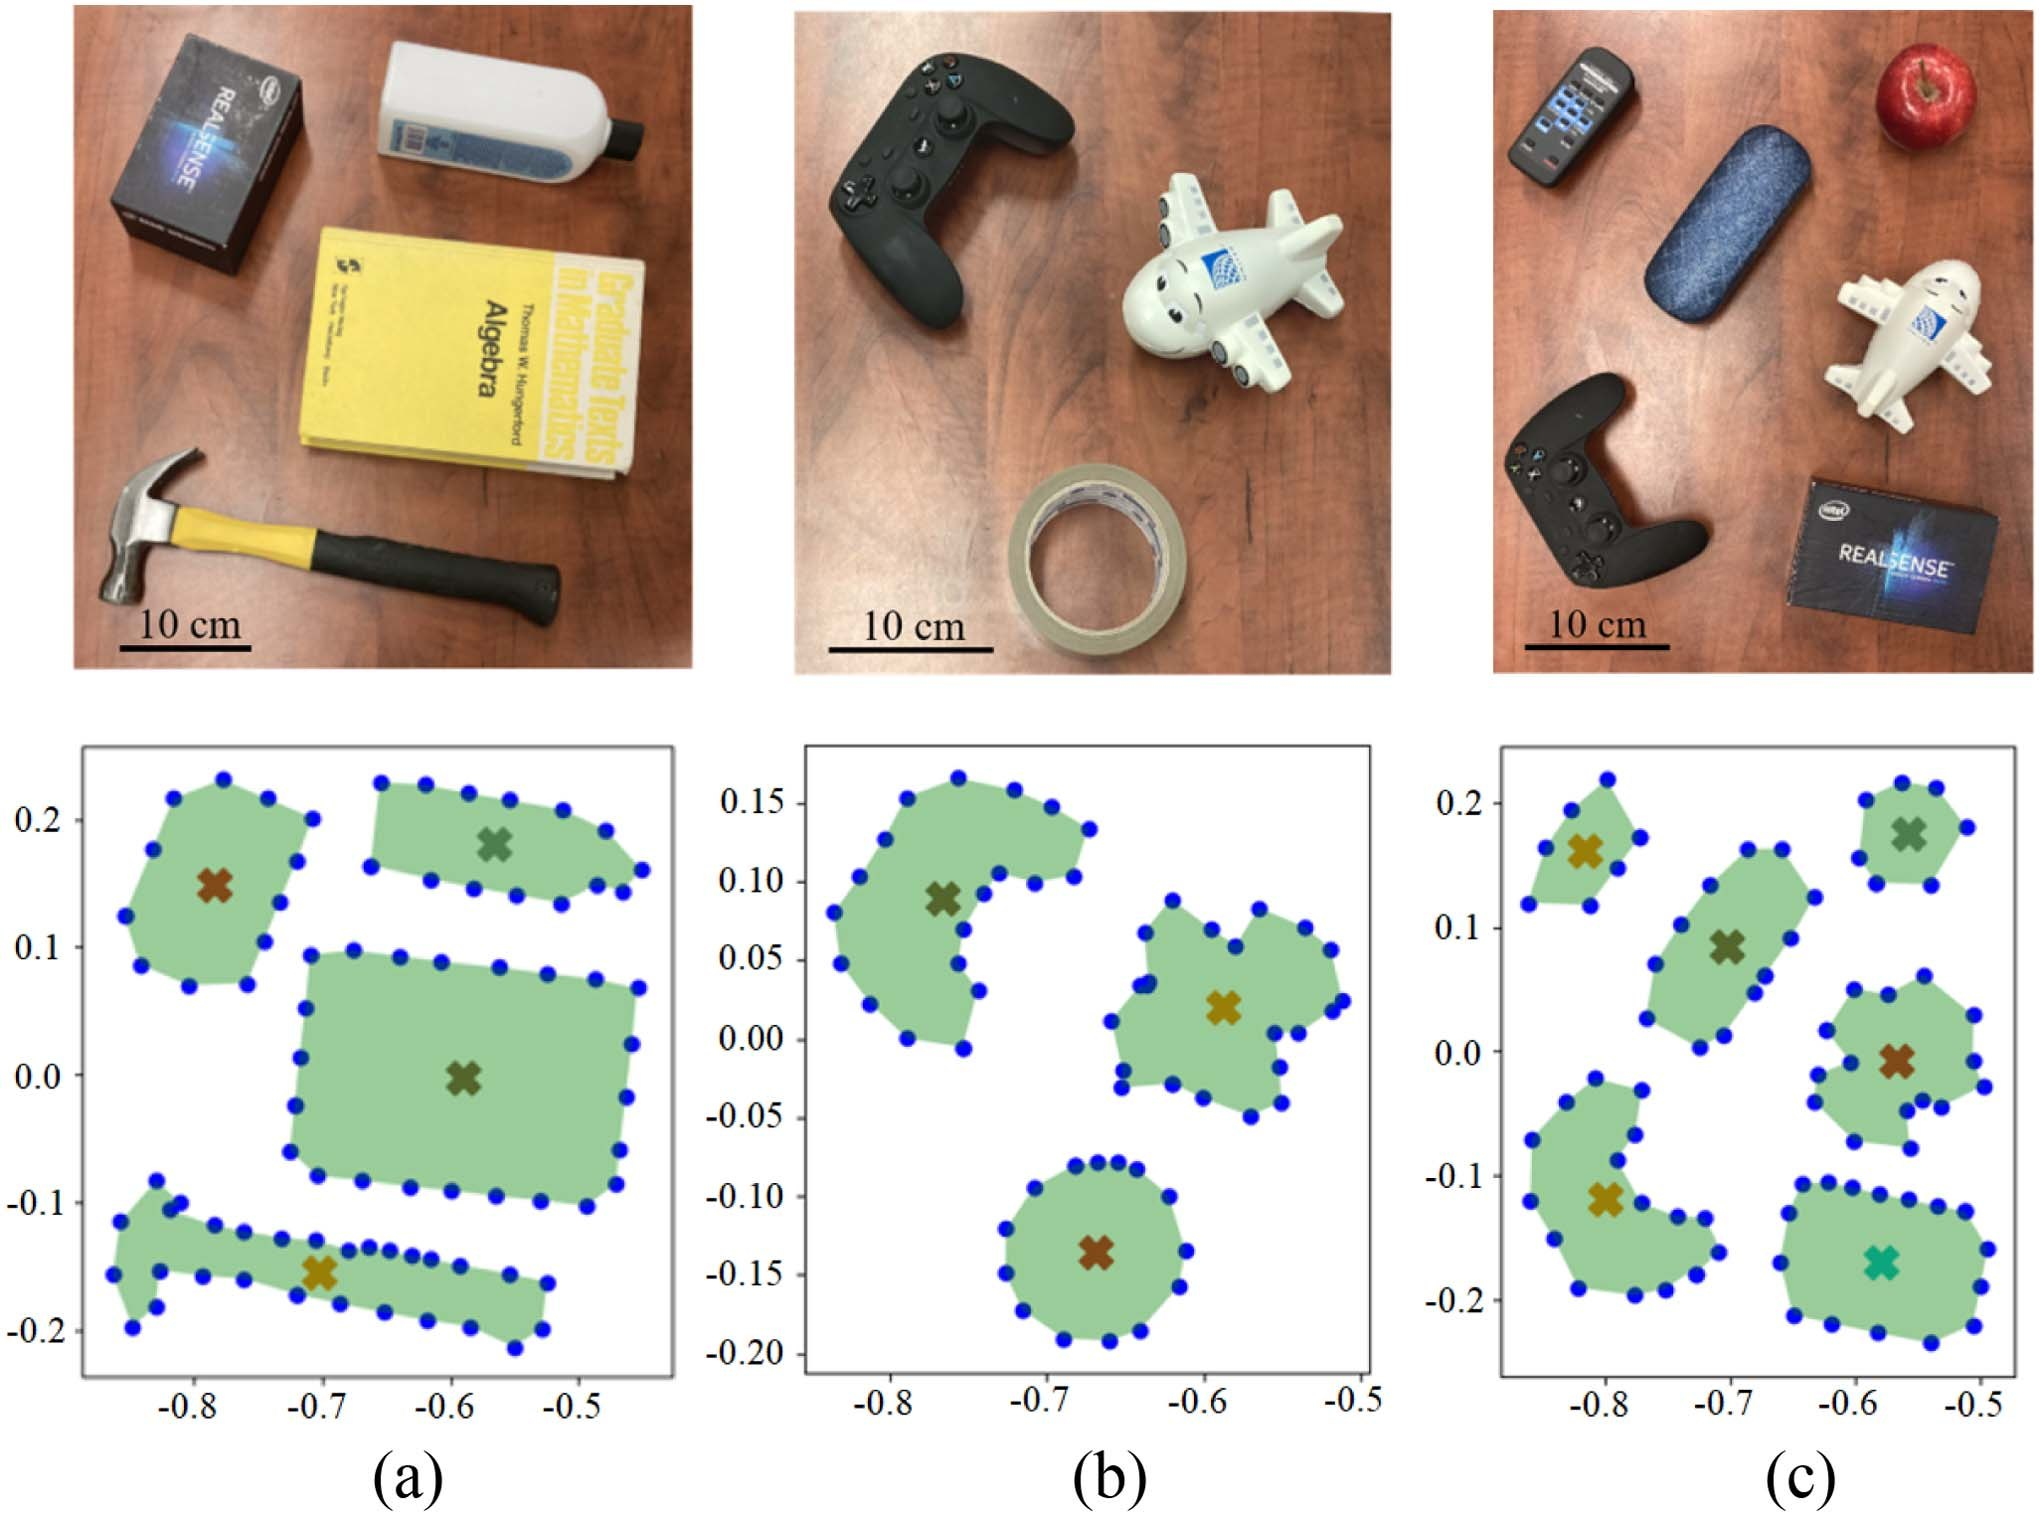
\includegraphics[width=\textwidth]{figures/related-works-2-results}
            \caption{Results of active tactile exploration in real experiments., from~\cite{Xiao_2022}}
        \end{figure}
    \end{column}
\end{columns}